\documentclass[12pt]{article}
\usepackage[a4paper,margin=1in]{geometry}
\usepackage{booktabs}
\usepackage{array}
\usepackage{hyperref}
\usepackage{graphicx}
\hypersetup{colorlinks=true,linkcolor=black,urlcolor=blue}

\title{Tugas Implementasi Deep Learning 1}
\author{Dzikran Azka Sajidan\\NIM 23/516665/PA/22110}
\date{\href{https://github.com/SjdnDzikran/tugas-deep-learning-1}{https://github.com/SjdnDzikran/tugas-deep-learning-1}}

\begin{document}
\maketitle

\section*{Pendahuluan}
Tugas ini mengevaluasi jaringan syaraf tiruan yang diimplementasikan dari awal dengan NumPy untuk memprediksi risiko stroke pada dataset Stroke Prediction dari Kaggle. Dataset terdiri atas 5.110 observasi setelah pembersihan awal, dengan 16 fitur hasil encoding serta rasio kelas positif sekitar 4,9\% pada kedua himpunan latih dan uji, menandakan masalah ketidakseimbangan kelas yang perlu diperhatikan selama pelatihan.

\section*{Metodologi}
Pra-pemrosesan meliputi pengisian nilai BMI yang hilang menggunakan median, penghapusan kategori gender langka, one-hot encoding fitur kategorikal, standardisasi fitur numerik, dan pembagian data 80:20 dengan stratifikasi label. Jaringan menggunakan arsitektur \([\texttt{input\_dim},32,16,1]\) dengan aktivasi sigmoid pada lapisan keluaran dan variasi sigmoid, tanh, serta ReLU pada lapisan tersembunyi. Tiga strategi optimisasi diuji: batch, mini-batch (32), dan stochastic gradient descent. Semua model dilatih selama 200 epoch dengan laju belajar tetap 0{,}01.

\begin{table}[htbp]
    \centering
    \caption{Ringkasan dataset setelah pra-pemrosesan.}
    \begin{tabular}{>{\raggedright\arraybackslash}p{0.52\textwidth} >{\raggedleft\arraybackslash}p{0.35\textwidth}}
        \toprule
        Aspek & Nilai \\
        \midrule
        Jumlah sampel & 5.110 \\
        Ukuran himpunan latih (batch penuh) & 4.087 \\
        Ukuran himpunan uji (estimasi) & 1.023 \\
        Jumlah fitur numerik + hasil encoding & 16 \\
        Proporsi kelas positif (latih / uji) & 0,049 / 0,049 \\
        \bottomrule
    \end{tabular}
\end{table}

\section*{Hasil dan Diskusi}
Evolusi loss dan akurasi selama pelatihan ditunjukkan pada Gambar~\ref{fig:loss-accuracy}, menegaskan bahwa model dengan optimisasi stochastic gradient descent mencapai konvergensi tercepat dan stabil dibandingkan dua strategi lainnya. Tabel~\ref{tab:metrics} merangkum performa sembilan kombinasi aktivasi dan strategi gradient descent. Kombinasi sigmoid dengan stochastic gradient descent menghasilkan F1-score tertinggi sebesar 0,171 dan presisi 0,30, walaupun recall masih terbatas (0,12). Variasi tanh dengan stochastic gradient descent berada di peringkat kedua dengan F1-score 0,16 dan keseimbangan presisi-recall yang serupa. Strategi batch cenderung menghasilkan gradien yang stabil namun gagal mengenali kelas minoritas (F1-score 0), menandakan kebutuhan teknik penyeimbangan tambahan. Mini-batch menawarkan kompromi yang baik, terutama untuk aktivasi tanh, namun masih menghadapi tantangan pada recall karena ketidakseimbangan data.

\begin{figure}[htbp]
    \centering
    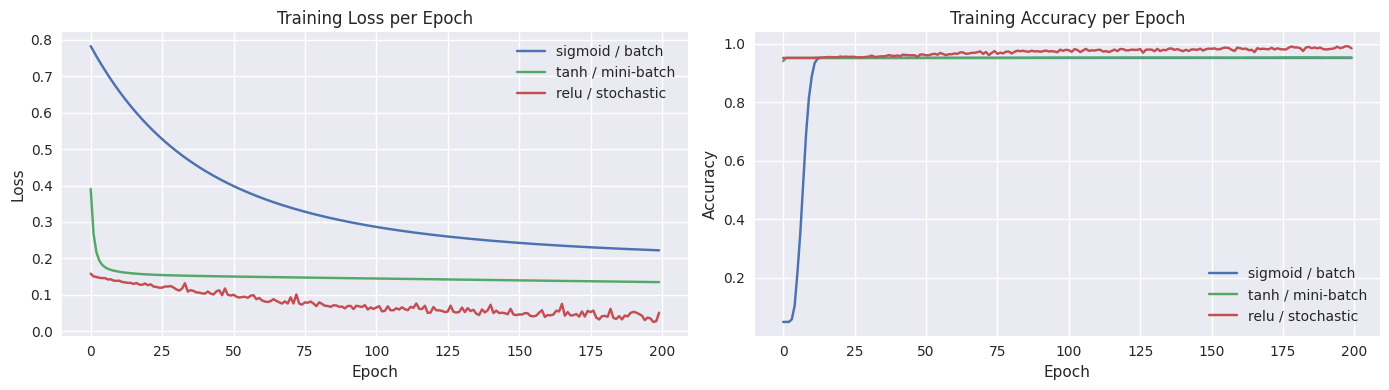
\includegraphics[width=1\textwidth]{loss-and-traning-accuracy.png}
    \caption{Kurva loss dan akurasi pelatihan untuk tiga strategi gradient descent.}
    \label{fig:loss-accuracy}
\end{figure}

\begin{table}[htbp]
    \centering
    \caption{Kinerja model pada data uji untuk setiap kombinasi aktivasi dan strategi gradient descent.}
    \label{tab:metrics}
    \small
    \begin{tabular}{llrrrrrr}
        \toprule
        Aktivasi & Strategi & \multicolumn{1}{c}{Train Loss} & \multicolumn{1}{c}{Test Loss} & \multicolumn{1}{c}{Akurasi} & \multicolumn{1}{c}{Presisi} & \multicolumn{1}{c}{Recall} & \multicolumn{1}{c}{F1} \\
        \midrule
        Sigmoid & Batch & 0{,}222 & 0{,}222 & 0{,}951 & 0{,}000 & 0{,}000 & 0{,}000 \\
        Sigmoid & Mini-batch & 0{,}162 & 0{,}163 & 0{,}951 & 0{,}000 & 0{,}000 & 0{,}000 \\
        Sigmoid & Stochastic & \textbf{0{,}119} & 0{,}199 & 0{,}943 & \textbf{0{,}300} & \textbf{0{,}120} & \textbf{0{,}171} \\
        Tanh & Batch & 0{,}308 & 0{,}305 & 0{,}951 & 0{,}000 & 0{,}000 & 0{,}000 \\
        Tanh & Mini-batch & 0{,}135 & \textbf{0{,}165} & \textbf{0{,}954} & 1{,}000 & 0{,}060 & 0{,}113 \\
        Tanh & Stochastic & \textbf{0{,}005} & 0{,}579 & 0{,}918 & 0{,}160 & 0{,}160 & 0{,}160 \\
        ReLU & Batch & 0{,}228 & 0{,}228 & 0{,}951 & 0{,}000 & 0{,}000 & 0{,}000 \\
        ReLU & Mini-batch & 0{,}133 & 0{,}168 & 0{,}952 & 1{,}000 & 0{,}020 & 0{,}039 \\
        ReLU & Stochastic & 0{,}051 & 0{,}654 & 0{,}930 & 0{,}077 & 0{,}040 & 0{,}053 \\
        \bottomrule
    \end{tabular}
\end{table}

 
\section*{Kesimpulan}
Eksperimen menunjukkan bahwa implementasi jaringan syaraf tiruan dari awal mampu mencapai F1-score 0,171 pada data uji dengan kombinasi sigmoid dan stochastic gradient descent. Namun, ketidakseimbangan kelas tetap menjadi faktor pembatas utama bagi recall. Pekerjaan lanjutan dapat mencakup penyeimbangan kelas (mis.~SMOTE atau penyesuaian bobot kelas), eksplorasi laju belajar adaptif, atau regulasi tambahan untuk meningkatkan generalisasi terhadap kelas minoritas.

\end{document}
